\setcounter{section}{4}
\section{GIÁ TRỊ LƯỢNG GIÁC CỦA MỘT GÓC TỪ $0^\circ$ ĐẾN $180^\circ$}
\subsection{TÓM TẮT LÝ THUYẾT}

\subsubsection{Giá trị lượng giác của một góc}
\begin{itemize}
	\item [\iconMT] \indam{Định nghĩa:} Với mỗi góc $\alpha$ $(0^\circ\le \alpha \le 180^\circ )$, ta xác định duy nhất một điểm $M$ trên nửa đường tròn đơn vị sao cho $\widehat{xOM}=\alpha $. Giả sử điểm $M$ có tọa độ $M(x_0;y_0 )$, khi đó ta có định nghĩa:
	\begin{gachsoc}
	\immini{\begin{itemize}
			\item  sin của góc $\alpha $ là $y_0$, kí hiệu $\sin \alpha$. 
			\item  cosin của góc $\alpha $ là $x_0$, kí hiệu $\cos \alpha$.
			\item tang của góc $\alpha $ là $\dfrac{y_0}{x_0}\,\,(x_0\ne 0 )$ ,
			kí hiệu $\tan \alpha$. 
			\item cotang của góc $\alpha $ là $\dfrac{x_0}{y_0}\,\,(y_0\ne 0 )$, kí hiệu $\cot \alpha$.
		\end{itemize} 
	}{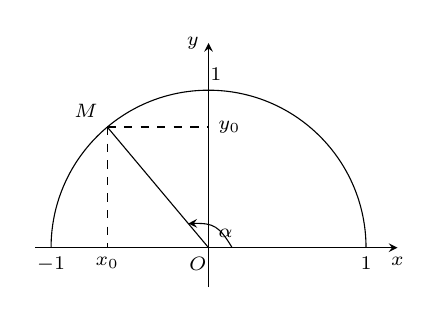
\begin{tikzpicture}[>=stealth,font=\scriptsize]
			\draw[->] (-2.2,0) -- (2.4,0) node[below]{$x$};
			\draw[->] (0,-.5) -- (0,2.6) node[left]{$y$};
			\draw (.1,0) node[below left]{$O$}
			(-2,0) node[below]{$-1$}
			(2,0) node[below]{$1$}
			(-0.1,2) node[above right]{$1$};
			\draw (2,0) arc (0:180:2cm);
			\path (130:2cm) coordinate (M);
			\draw[dashed] (M) node[above left]{$M$} -- (M|- 0,0) node[below]{$x_0$};
			\draw[dashed] (M) -- (M -|0,0) node[right]{$y_0$};
			\draw (0,0) -- (M);
			\draw[->] (0.3,0) to [bend right,looseness=1.3] (130:0.4cm) node[above right,midway]{$\alpha$};
	\end{tikzpicture}}
	\end{gachsoc}
\indamm{Từ định nghĩa trên, ta có:}
\begin{tcolorbox}[colframe=orange,colback=white,boxrule=0.2mm]
	\begin{listEX}[3]
		\item [\ding{172}] $\tan \alpha=
		\dfrac{\sin\alpha}{\cos\alpha}$
		\item [\ding{173}]  $\cot \alpha=
		\dfrac{\cos\alpha}{\sin\alpha}$
		\item [\ding{174}] $\tan \alpha=\dfrac{1}{\cot\alpha}$
	\end{listEX}
\end{tcolorbox}
	\item [\iconMT] \indam{Bảng giá trị lượng giác của góc đặc biệt:}
	\begin{center}
		\renewcommand{\arraystretch}{2}
		\begin{tabular}{|c|c|c|c|c|c|c|}
			\hline
		 & $0^\circ$ & $30^\circ$ & $45^\circ$ & $60^\circ$ & $90^\circ$ & $180^\circ$\\
			\hline
			$\sin \alpha$  & $0$ & $\dfrac{1}{2}$ & $\dfrac{\sqrt{2}}{2}$ & $\dfrac{\sqrt{3}}{2}$ & $1$ & $0$\\
			\hline
			$\cos \alpha$  & $1$ & $\dfrac{\sqrt{3}}{2}$ & $\dfrac{\sqrt{2}}{2}$ & $\dfrac{1}{2}$ & $0$ & $-1$\\
			\hline
			$\tan \alpha$ & $0$ & $\dfrac{1}{\sqrt{3}}$ & $1$ & $\sqrt{3}$ & $\big|\big|$ & $0$\\
			\hline
			$\cot \alpha$ & $\big|\big|$ & $\sqrt{3}$ & $1$ & $\dfrac{1}{\sqrt{3}}$ & $0$ & $\big|\big|$\\
			\hline
		\end{tabular}
	\end{center}
\end{itemize}
\subsubsection{Mối quan hệ giữa các giá trị lượng giác}
\begin{itemize}
	\item [\iconMT] \indam{Hai góc bù nhau:} Trên hình bên ta có dây cung $NM$ song song với trục $Ox$ và nếu $\widehat{xOM}=\alpha $ thì $\widehat{xON}=180^\circ-\alpha $. Ta có $y_{M}=y_{N}=y_0,$ $x_{M}=-x_{N}=x_0$. Do đó
	\begin{gachsoc}	
			\immini{
			\begin{listEX}[1]
			\item [\ding{172}] $\sin (180^\circ-\alpha )=\sin \alpha$
			\item [\ding{173}] $\cos (180^\circ-\alpha )=-\cos \alpha$
			\item [\ding{174}] $\tan (180^\circ-\alpha )=-\tan \alpha$
			\item [\ding{175}] $\cot (180^\circ-\alpha )=-\cot \alpha$
		\end{listEX}
	}{\begin{tikzpicture}[scale=1, font=\footnotesize,>=stealth,x=2cm,y=2cm]
			\def\x{0.715}
			\def\a{44}
			\pgfmathsetmacro{\y}{\x*tan(\a)}
			\draw[->] (-1.3,0)--(1.3,0) node [below]{$x$};
			\draw[->] (0,-0.2)--(0,1.3) node [left]{$y$};
			\node at (0,0) [below left]{$O$};
			\draw (1,0) arc (0:180:2cm);
			\fill (1,0) node[below]{$1$} circle(1pt);
			\fill (-1,0) node[below]{$-1$} circle(1pt);
			\fill (0,1) node[above left]{$1$} circle(1pt);
			\fill (\x,0) node[below]{$x_0$} circle(1pt);
			\fill (-\x,0) node[below]{$-x_0$} circle(1pt);
			\fill (\a:1) node[above right]{$M$} circle(1pt);
			\fill (180-\a:1) node[above left]{$N$} circle(1pt);
			\fill (0,\y) node[above right]{$y_0$} circle(1pt);
			\draw[dashed] (\x,0)|-(0,\y);
			\draw[dashed] (-\x,0)|-(0,\y);
			\draw (44:1)--(0,0)--(136:1);
			\draw (0.3,0) arc (0:\a:0.6cm);
			\node at (0,0)[shift={(25:0.2)}]{\tiny{$\alpha$}};
			\draw (0.2,0) coordinate (A) -- (0,0) coordinate (B) -- (136:0.6 cm) coordinate (C) pic [draw, double, angle radius = 9mm] {angle = A--B--C}; 
			\draw (0.25,0.55)node{\tiny{$180^\circ-\alpha$}};
	\end{tikzpicture}}
		\end{gachsoc}
	\item [\iconMT] \indam{Hai góc phụ nhau:} Hình vẽ bên, hai điểm $M$ và $N$ ứng với hai góc phụ nhau $\alpha$ và $90^\circ-\alpha$ ($\widehat{xOM}=\alpha$, $\widehat{xON}=90^\circ-\alpha$ )
	\begin{gachsoc}
		\immini{	\begin{itemize}
				\item [$\bullet$] $\cos \left( 90^\circ-\alpha  \right) = \sin \alpha$
				\item [$\bullet$] $\sin \left(90^\circ-\alpha  \right) = \cos \alpha$
				\item [$\bullet$] $\tan \left(90^\circ-\alpha  \right) = \cot \alpha$
				\item [$\bullet$] $\cot \left( 90^\circ-\alpha  \right) = \tan \alpha$
			\end{itemize}
		}{
			\begin{tikzpicture}[scale=1, font=\footnotesize,>=stealth,x=2cm,y=2cm]
				\def\x{0.866}
				\def\a{30}
				\pgfmathsetmacro{\y}{\x*tan(\a)}
				\draw[->] (-1.3,0)--(1.3,0) node [below]{$x$};
				\draw[->] (0,-0.2)--(0,1.3) node [left]{$y$};
				\node at (0,0) [below left]{$O$};
				\draw (1,0) arc (0:180:2cm);
				\fill (1,0) node[below]{$1$} circle(1pt);
				\fill (-1,0) node[below]{$-1$} circle(1pt);
				\fill (0,1) node[above left]{$1$} circle(1pt);
				\fill (\x,0) node[below]{$x_0$} circle(1pt);
				\fill (\a:1) node[above right]{$M$} circle(1pt);
				\fill (90-\a:1) node[above right]{$N$} circle(1pt);
				\fill (0,\y) node[above left]{$y_0$} circle(1pt);
				\draw[dashed] (\x,0)|-(0,\y);
				\draw[dashed] (\y,0)|-(0,\x);
				\draw (\a:1)--(0,0)--(90-\a:1);
				\draw (0.3,0) arc (0:\a:0.6cm);
				\node at (0,0)[shift={(15:0.25)}]{\tiny{$\alpha$}};
				\draw (0.2,0) coordinate (A) -- (0,0) coordinate (B) -- (90-\a:0.6 cm) coordinate (C) pic [draw, double, angle radius = 9mm] {angle = A--B--C}; 
				\draw (0.55,0.3)node{\tiny{$90^\circ-\alpha$}};
		\end{tikzpicture}}
	\end{gachsoc}
\end{itemize}

\subsection{RÈN LUYỆN KĨ NĂNG GIẢI TOÁN}
\begin{dang}{Giá trị lượng giác của góc $\alpha$ cho trước ($0^\circ\le \alpha \le 180^\circ$)}
\end{dang}
	\begin{vd}
		Bằng cách vẽ nửa đường tròn đơn vị, hãy tính các giá trị lượng giác của góc $\alpha$ với
		\begin{tasks}(4)
			\task $\alpha=60^\circ$.
			\task $\alpha=90^\circ$.
			\task $\alpha=120^\circ$.
			\task $\alpha=135^\circ$.
		\end{tasks}
	\end{vd}
	\begin{vd}
		Bằng cách vẽ nửa đường tròn đơn vị, hãy tìm góc $\alpha$ ($0^\circ\le \alpha \le 180^\circ$) trong các trường hợp sau:
		\begin{tasks}(4)
			\task $\cos\alpha=-\dfrac{\sqrt{2}}{2}$.
			\task $\cos\alpha=\dfrac{1}{2}$.
			\task $\sin\alpha=\dfrac{\sqrt{2}}{2}$.
			\task $\sin\alpha=1$.
		\end{tasks}
	\end{vd}
\begin{vd}
	Trên mặt phẳng toạ độ $Oxy$, lấy điểm $M$ thuộc nửa đường tròn đơn vị sao cho $\widehat{xOM}=120^{\circ}$. Gọi $N$ là điểm đối xứng với $M$ qua trục tung. Tính giá trị của $\tan\widehat{xON}$.
	\loigiai{
	Ta có $\widehat{xOM}$ và $\widehat{xON}$ là hai góc bù nhau nên $\widehat{xON}=180^\circ-120^\circ=60^\circ$.\\
	Suy ra $\tan\widehat{xON}=\tan 60^\circ =\sqrt{3}$.
	}
\end{vd}
\begin{dang}{Tính giá trị biểu thức}
\end{dang}
\begin{vd}%[0H2Y1]
	Tính giá trị biểu thức sau
	\begin{tasks}(2)
		\task $A= 2\cos 30^\circ+3\sin 120^\circ$.
		\task $B=a\cos60^{\circ}+2a\tan45^{\circ}-3a\sin30^{\circ}$.
	\end{tasks}
	\loigiai{
		\begin{enumerate}[a)]
			\item
			\item Ta có $B=\dfrac{1}{2}a+2a-\dfrac{1}{2}.3a=a$.
		\end{enumerate}
		
	}
\end{vd}
\begin{vd}%[0H2Y1]
	Cho $x=30^{\circ}$. Tính $A=\sin (2x)-3\cos x$.
	\loigiai{
		$A=\sin 2.(30^{\circ})-3\cos30^{\circ}=\sin60^{\circ}-3\cos30^{\circ}=\dfrac{\sqrt{3}}{2}-3\dfrac{\sqrt{3}}{2}=-\sqrt{3}$.
	}
\end{vd}

\begin{vd}
	Biết $\sin15^\circ=\dfrac{\sqrt{3}-1}{2\sqrt{2}}$. Tính giá trị biểu thức $P=\sin165^\circ+\cos75^\circ$.
\end{vd}

\begin{vd}%[0H2K1]
	Tính giá trị các biểu thức sau:
	\begin{tasks}(1)
		\task $A=\sin^2 10^{\circ}+\sin^2 20^{\circ}+\dots+\sin^2 170^{\circ}+\sin^2 180^{\circ}$.
		\task $B=\tan 10^{\circ}.\tan 20^{\circ}\dots\tan 80^{\circ}$.
		\task $C=\cot 20^{\circ}+\cot 40^{\circ}+\dots +\cot 140^{\circ}+\cot160^{\circ}$.
	\end{tasks}
	\loigiai{
		\begin{enumerate}[a)]
			\item Ta có $\sin 10^{\circ}=\sin170^{\circ},\ \sin20^{\circ}=\sin160^{\circ},\dots$, suy ra $C= 2\bigl(\sin^2 10^{\circ}+\sin^2 20^{\circ}+\dots+\sin^2 80^{\circ}\bigr)+\sin^2 90^{\circ}$. Mặt khác ta có $\sin 80^{\circ}=\cos 10^{\circ},\ \sin 70^{\circ}=\cos 20^{\circ},\dots$, có 4 cặp như vậy nên ta tính được $A=5$.
			\item $\tan 10^{\circ}=\cot 80^{\circ}$, $\tan 20^{\circ}=\cot 70^{\circ}$, $\tan 30^{\circ}=\cot 60^{\circ}$, $\tan 40^{\circ}=\cot 50^{\circ}$. Do đó, ta tính được $B=1$.
			\item $\cot20^{\circ}=-\cot160^{\circ},\ \cot40^{\circ}=-\cot140^{\circ},\dots$ nên ta tính được $C=0$.
		\end{enumerate}
	}
\end{vd}
\begin{dang}{Rút gọn, chứng minh biểu thức}
\end{dang}
	\begin{vd}
		Chứng minh rằng với mọi góc $\alpha$ ($0^\circ< \alpha < 180^\circ$), ta đều có
		\begin{tasks}(3)
			\task $\sin^2\alpha + \cos^2\alpha =1$.
			\task $1+\tan^2\alpha=\dfrac{1}{\cos^2\alpha}$.
			\task $1+\cot^2\alpha=\dfrac{1}{\sin^2\alpha}$.
		\end{tasks}
	\end{vd}

	\begin{vd}
	Áp dụng kết quả của \indamm{Ví dụ 7}, hãy giải các bài toán sau:
	\begin{tasks}(1)
		\task Cho $\sin\alpha = \dfrac{3}{5}$. Tính giá trị của biểu thức $A=2\sin^2\alpha+3\cos^2\alpha$.
		\task Cho $\tan\alpha = 2$. Tính giá trị của biểu thức 
		\begin{enumEX}[*]{2}
			\item $B=\dfrac{2\sin\alpha+3\cos\alpha}{5\sin\alpha+\cos\alpha}$.
			\item $C=\dfrac{\sin\alpha+\cos\alpha}{3\sin^3\alpha+\cos^3\alpha}$.
		\end{enumEX}
	\end{tasks}
	
	\end{vd}

	\begin{vd}%[0H2B1]
	Cho $A, B, C$ là các góc của tam giác. Chứng minh các đẳng thức sau:
	\begin{tasks}(2)
		\task $\sin\left(A+B\right)=\sin C.$
		\task $\cos\left(A+B\right)+\cos C=0.$
		\task $\sin\dfrac{A+B}{2}=\cos\dfrac{C}{2}.$
		\task $\tan\left(A-B+C\right)=-\tan2B.$
	\end{tasks}
	\loigiai{ Do $A, B, C$ là các góc của tam giác nên ta có $A+B+C=180^{\circ}$.
		\begin{enumerate}[a)]
			\item Ta có $A+B+C=180^{\circ}\Leftrightarrow A+B=180^{\circ}-C.$\\
			Từ đó suy ra $\sin\left(A+B\right)=\sin \left(180^{\circ}-C\right)=\sin C.$
			\item Ta có $A+B+C=180^{\circ}\Leftrightarrow A+B=180^{\circ}-C.$\\
			Từ đó suy ra $\cos\left(A+B\right)=\cos \left(180^{\circ}-C\right)=-\cos C \Rightarrow \cos\left(A+B\right)+\cos C=0.$
			\item Ta có $A+B+C=180^{\circ}\Leftrightarrow \dfrac{A+B}{2}=\dfrac{180^{\circ}-C}{2}=90^{\circ}-\dfrac{C}{2}.$\\
			Từ đó suy ra $\sin\dfrac{A+B}{2}=\sin\left(90^{\circ}-\dfrac{C}{2}\right)= \cos\dfrac{C}{2}.$
			\item Ta có $\tan\left(A-B+C\right)=\tan\left(A+B+C-2B\right)=\tan\left(180^{\circ}-2B\right)=-\tan2B.$
		\end{enumerate}
	}
	\end{vd}